%%%%%%%%%%%%%%%%%%%%%%%%%%
\chapter{Polyphonic Sound Event Detection}
\label{ch:polySED}

Sound event detection (SED) algorithms in a real-life scenario face many challenges. These include  environmental noise, events of the same class produced by different sources (i.e., intra-class variability) and simultaneous events. In particular, since multiple events are very likely to overlap, a \textit{polyphonic} SED algorithm, i.e., an algorithm able to detect multiple simultaneous events, needs to be designed. A polyphonic SED algorithm can be considered as system which is able to perform contemporary detection - determining the starting and ending point of multiple events - and classification - assigning a label to each of the sound events occurring in the audio stream. In this chapter we show two algorithms for polyphonic SED in real life audio. The first is based on a two-step algorithm: the detection task is performed by an adaptive energy Voice Activity Detector (VAD) system, while the active-event classification is acted by a deep neural network. The second system is a fully data-driven approach which is totally based on the CapsNet deep neural architecture presented by Sabour et al. \cite{sabour2017dynamic}. 
\vspace{-0.5cm}
\section{Sound Event Detection in Real Life Audio - DCASE 2016}
\label{sec:sed_dcase2016}
In this section we present and compare two neural-based algorithms designed for sound event detection in real life audio. Both systems have been developed and evaluated with the material provided for the third task of the Detection and Classification of Acoustic Scenes and Events (DCASE) 2016 challenge. For the first algorithm, we make use of an artificial neural network trained on different features extracted from the down-mixed Monaural-channel audio. Secondly, we analyse a binaural algorithm where the same feature extraction is performed on four different channels: the two binaural channels, the averaged Monaurall signal and the difference between the binaural channels. The proposed feature set comprehends, along with mel-frequency cepstral coefficients and log-mel energies, also activity information extracted with two different voice activity detection (VAD) algorithms.

\subsection{Introduction}

In occasion of the DCASE 2016, many novel systems featuring recurrent neural networks (RNNs) and multilayer perceptrons (MLPs) have been proposed, even though only one of them~\cite{adavanne2016sound} managed to outperform the baseline system (based on a GMM) thus reaching the first rank in the challenge third task. In our opinion, this proves that there is still a lot of space for research in approaching SED with ANNs, therefore we here propose a system which relies on a voice activity detection (VAD) algorithm for the detection of acoustic events which are then classified by an ANN. During our experiments we compare different well-established audio representation, \emph{i.e.,}\ log-mel energies and mel-frequency cepstral coefficients (MFCCs), extracted in both monaural and binaural configuration. Moreover, we will evaluate two VAD algorithms (\emph{i.e.,}\ adaptive energy (AE) and Sohn's VAD), as well as two different ANN architectures for classification, \emph{i.e.,}\ MLPs and RNNs. Our aim is therefore to give a novel contribution by presenting a robust system capable to improve the results obtained by participants to the DCASE 2016 challenge.


\subsection{Proposed method}

As we can see from \figref{fig:system_scheme} it is possible to divide the system functioning into two phases: training and testing. During training we do not need to use any algorithm for event detection, since onset and offset instants are already provided in the ground truth, therefore we can simply train an ANN to recognise the different events. At test time, on the other hand, onset and offset instants are not given, therefore we firstly make use of a VAD algorithm for determining them, and secondly we feed the corresponding audio sequences to the ANN classifier.

\begin{figure}[h]
	\centering
	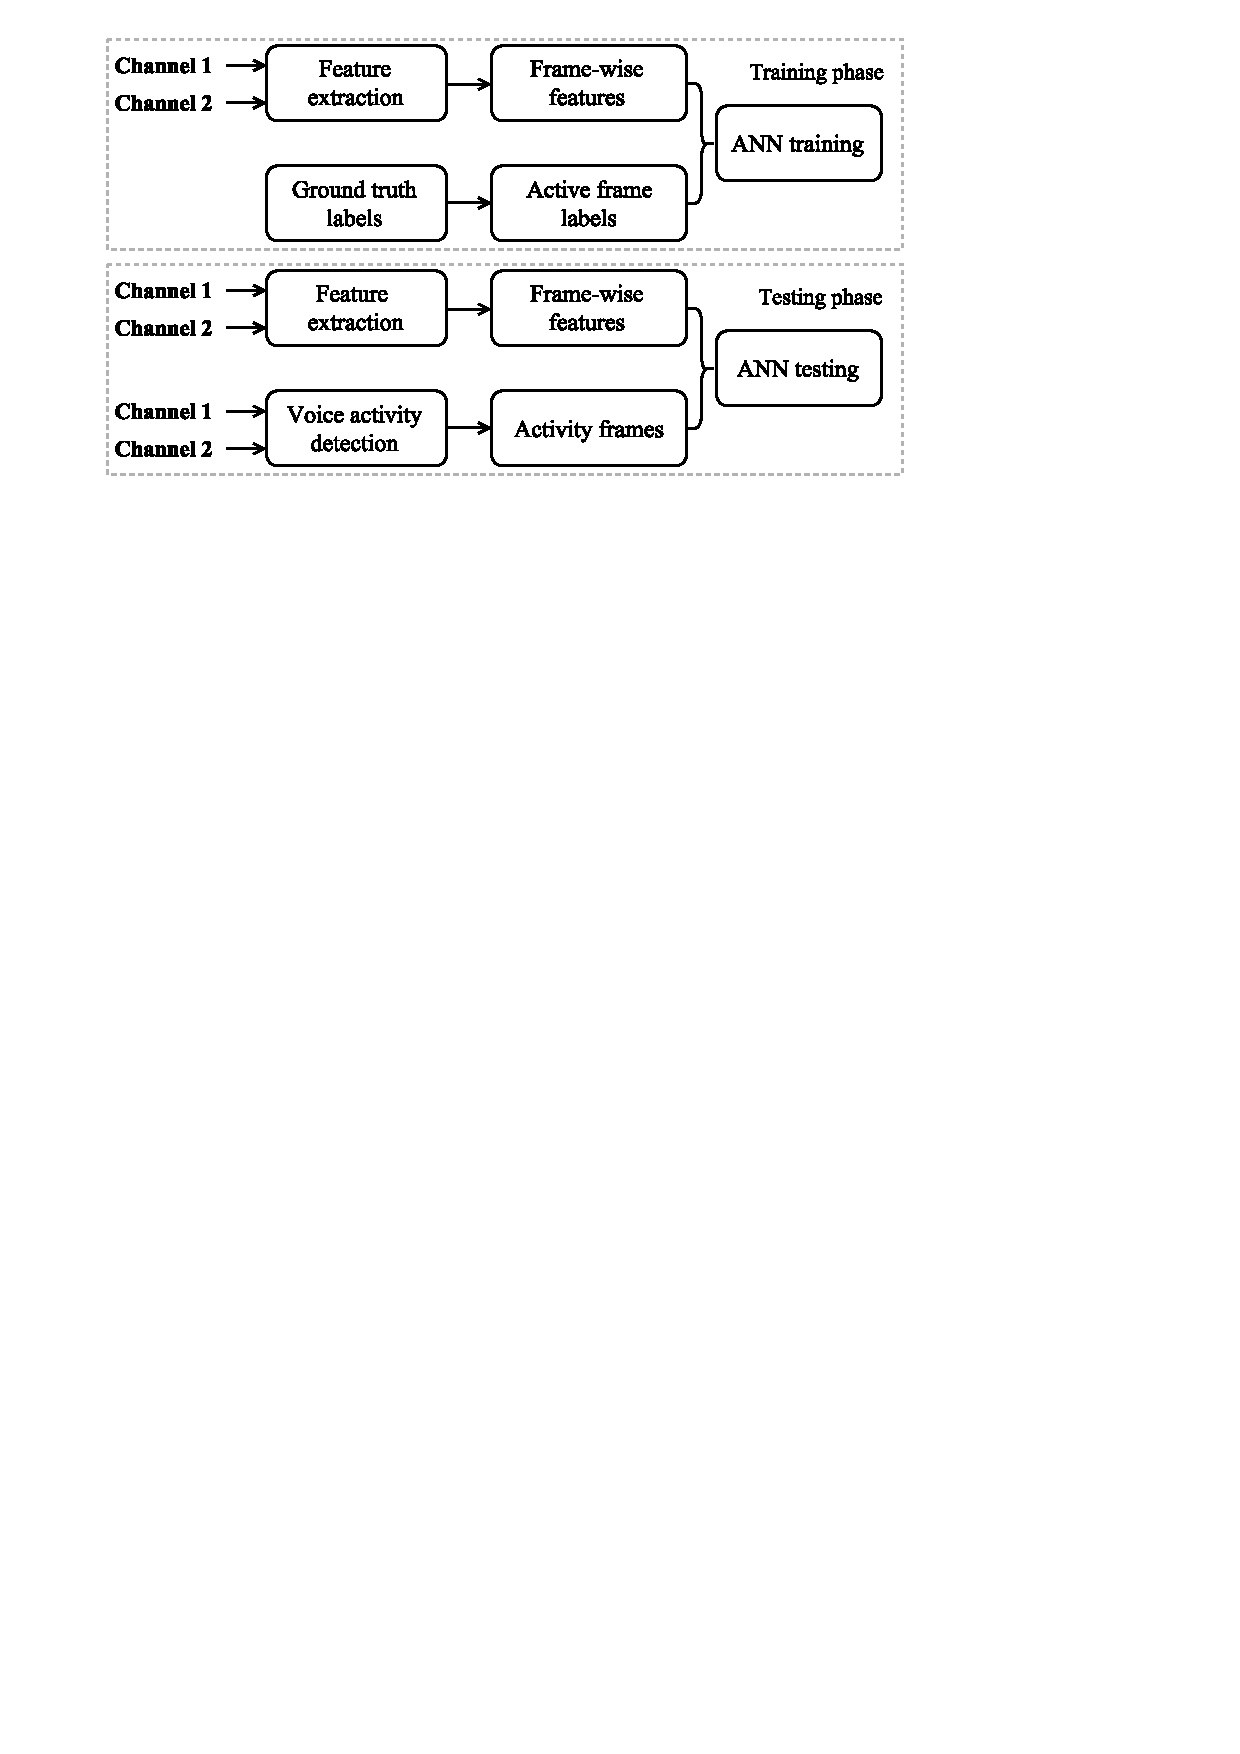
\includegraphics[width=0.7\textwidth]{img/system_scheme.pdf}
	\caption[Sound Event Detection - DCASE 2016]{Block diagram of training and testing phases. At test time a VAD algorithm is used to determine onset and offset instants of the detected events.}
	\label{fig:system_scheme}
\end{figure}

\subsubsection{Feature representations}

In order to perform the SED task with ANNs, a set of one or more audio representations have been extracted from the raw audio signal. Aiming to evaluate the impact of binaural information on the classification performance, we will, in the first instance, distinguish the proposed sets between monaural and binaural feature sets. We highlight that, for all the extracted feature sets, a frame-wise short-time Fourier transform (STFT) is firstly applied to the audio signal on frame windows of 40 ms with 50\% overlap. Moreover, all feature extraction processes described hereafter have been performed with openSMILE~\cite{eyben2013recent}, a license-free software package developed by the Technical University of Munich.

The first monaural set is known as log-mel spectrogram. In this case a down-mixing of the two audio channels is required before calculating the STFT coefficients. After the STFT coefficients are extracted, we apply a mel conversion of the frequency scale with a 26-bands mel-scale filter bank and compute the logarithm of all the energies so obtained. To complete the set, we also extract the first order delta coefficients operating on a context window of 10 frames. Given the log-mel coefficients and their respective deltas, this first set is composed of 52 coefficients for each frame.

The second monaural set is composed of another set of widely used features, that is mel-frequency cepstral coefficients (MFCCs). Starting from the same STFT coefficients previously obtained, we now compute the log-mel spectrogram with a 40-bands mel-scale filter bank. Then, we apply a 20-points discrete cosine transform (DCT) to each energy vector and, after excluding the 0\textsuperscript{th} order coefficient, we obtain a feature vector of 20 MFCCs. In order to complete the set, we also calculate the first and second order delta coefficients, therefore obtaining a 60-coefficients feature vector.

For the two binaural sets we decided to extract the log-mel (or the MFCC) features not only from the average of the two channels, but also from their difference and the two separate channels; this gives us a total of four channels. We decided to do so because, for example, if an important event is predominant in only one of the two channels, averaging them could lower the signal-to-noise ratio, thus increasing the system failure probability. For the first binaural set we extract the log-mel coefficients as for the first monaural set, but, given the presence of four channels, we now have a total of 108 coefficients for each frame. In order to avoid an excessive feature vector dimension, in this set we decide to avoid using the first and second order delta coefficients. Similarly, the second binaural set is obtained by extracting 20 MFCCs for each channel; since again we avoid using the delta coefficients, this leads us to a total of 80 coefficients for each frame. 

\subsubsection{Neural networks}

In this work two different ANNs architectures are tested for the SED problem, \emph{i.e.,}\ MLPs and RNNs.
The first layer of all proposed ANNs consists of a set of nodes to which the audio representation (taken on a frame scale) is applied, with the number of nodes varying from 52 to 108, depending on the chosen feature representation. The input is then propagated to the following three hidden layers, composed of 512 \textit{tanh} neurons each for MLPs and 54 rectifier neurons for RNNs.  Finally, the last layer of our networks is designed to output the class associated by the network with the given input. To do so, this layer is composed of a number of softmax neurons equal to the number of possible classes, \emph{i.e.,} 11 if we are dealing with a ``home'' scenario, and 7 in case of a ``residential area'' (see ~\tableref{tab:classes}). We highlight that, in case of MLPs, we obtain one label for each frame, whereas RNNs are able to output one label also for a batch of sequent frames.

The standard algorithm used for training the proposed MLPs is the backpropagation (BP) algorithm, whereas for RNNs the ``BP through time'' is used. After a first feed-forward phase, in which a batch of input is propagated through the networks, these algorithms exploit the derivative ``chain rule'' to back-propagate the error computed at the output layer and sequentially update all neuron weights~\cite{rojas2013neural}.

\subsubsection{Sound event detection and classification}

At test time we want the system to detect and correctly classify as many acoustic events as possible occurring in raw audio files of 30 seconds. Since no onset nor offset instants are given, we decide to use VAD algorithms in order to detect these instants. With this intent, two different VAD algorithms have been tested, \emph{i.e.,}\ AE, and Sohn's VAD. 

The AE approach makes use of two energy thresholds in order to determine the starting and ending point of an event-active audio sequence, \emph{i.e.,}\ the ``mean plus variance'' (MPV) and the ``mean minus variance'' (MMV) thresholds. These thresholds are firstly calculated over all the training dataset and then used to extract information about events activity: whenever a frame's energy exceeds the MPV threshold an onset event is triggered, then the event detection remains positive until the energy content drops below the MMV threshold. 

Sohn's VAD~\cite{sohn1999statistical}, on the other hand, is a method based on a statistical modelling of the audio in the time-frequency domain, with the model parameters being estimated with a maximum likelihood (ML) method. With this technique, the decision regarding the event's activity is devolved to a comparison between the averaged log-likelihood ratio (containing the a-priori and a-posteriori signal-to-noise ratios) and a fixed threshold $\eta \in (0,1)$. 

Whenever an audio file is processed by one of the two VAD algorithms we are able to extract the starting and ending instants between which an audio event has (supposedly) occurred. Hence, we can feed the network with the feature representation of the corresponding frames and finally obtain the event classification. We remind that, in case of MLPs, we obtain one label for each frame, whereas RNNs are able to output only one label for the whole frame batch. Due to this, we need to average all MLP outputs so to obtain the event's acoustic label, while RNN's outputs will need no further processing.

\subsection{Experiments}


\subsubsection{Datasets and metrics}
\label{sec:dcase2016-dataset}
The data we use during our experiments consist of two datasets provided for the third task (SED in real life audio) of the DCASE 2016 challenge~\cite{mesaros2016tut}. 
The former dataset, called \emph{development dataset}, was at first provided in order to make all challengers able to compare their development results, while the latter, the \emph{evaluation dataset}, was used for the final evaluation of the submitted systems, so its ground truth was made public only a few weeks after the end of the challenge. These acoustic scenes were selected from the challenge organizers to represent common environments of interest in applications for safety and surveillance (outside home) and human activity monitoring or home surveillance \cite{mesaros2016tut}.

Both datasets contains recordings of 3-5 minutes divided into two different acoustic scenarios: ``home'' and ``residential area''. Specific classes for each scenario are reported in Table~\ref{tab:classes}. 

\begin{table}[h]
	\centering
	\begin{tabular}{l c l c}\toprule
		\emph{Home} & \emph{Occurrences} & \emph{Residential area} & \emph{Occurrences}\\
		\midrule
		rustling & 60 & banging & 23\\
		snapping & 57 & bird singing & 271\\
		cupboard & 40 & car passing by & 108\\
		cutlery & 76 & children shouting & 31\\
		dishes & 151 & people walking & 52 \\
		drawer & 51 & people speaking & 44\\
		glass jingling & 36 & wind blowing & 30\\
		object impact & 250\\
		people walking & 54\\
		washing dishes & 84\\
		water tap running & 47\\
		\bottomrule
	\end{tabular}
	\caption[Classes of DCASE 2016 task 3 dataset]{Classes and their occurrences for the ``home'' and ``residential area'' scenarios for the SED in real life audio task of the DCASE 2016 challenge.}
	\label{tab:classes}
\end{table}

The development dataset consists of 10 recordings for the ``home'' scenario, and 12 for the ``residential area'', and for both a four-folds cross-validation data splitting is provided by the organizers of the challenge. While creating the cross-validation folds, the challenge organizers imposed the only condition that the test subset does not contain classes unavailable in training subset, therefore the class distribution between the test subsets is not assumed to be uniform.
The evaluation dataset contains 5 recordings for both the ``home'' and the ``residential area'' scenarios each. For this dataset no cross-validation is performed, so it is possible to train only one system with all the development dataset (including files previously meant for testing purpose) and then test it with the evaluation files.

Scores used to evaluate all systems are the well known F1 and error rate (ER) scores, which are used to evaluate the system over segments of one second. In obtaining the final score for the development dataset, we average the four per-fold scores as described in~\cite{mesaros2016tut}.

\subsection{Results}
\subsubsection{Experimental setup}

Concerning the network training, we initialize all weights according to a normal distribution with zero mean and 0.1 variance. We then train the networks following the adam~\cite{kingma2014adam} method for stochastic optimization, for which we keep the default hyper-parameter configuration. In order to prevent overfitting, for each fold we check the network performance on the respective fold's test set after each training epoch. If no improvement on this set is encountered for 60 consecutive epochs, the training is forced to an early stop.
After this phase we perform experiments on the evaluation data, for which we use the whole development training and test sets as training and validation data respectively. Then, at test time, we evaluate the system on the secret challenge data.

\subsubsection{Development results}

During our experiments we tested and compared different neural architectures, VAD algorithms, and feature representations. In \tableref{tab:dev_results_sohn} we report the results obtained with Sohn's VAD for 16 different system configurations, whereas in \tableref{tab:dev_results_ae} the same classifier and feature configurations are analysed in conjunction with AE VAD.

\tableref{tab:dev_results_sohn} highlights that the use of binaural audio features always enhances the system's performance in terms of both F1 and ER scores. Moreover, we can also notice that MLPs generally perform better than RNNs, in particular according to F1 scores, where no RNN manages to achieve more than 34.4\% F1 score. Finally, we report that the best system's configuration featuring Sohn's VAD is a MLP trained with binaural MFCC features, with a VAD threshold equal to 0.70. This system manages to reach 0.88 ER and 39.8\% F1 score, both averaged on the four folds.

\begin{table}[h]
	\centering
	\begin{tabular}{l c c c c}\toprule
		\emph{Features} & \emph{$\eta$} & \emph{Classifier} & \emph{ER} & \emph{F1} (\%)\\
		\midrule
		Monaural log-mel & 0.98 & MLP & 0.93 & 34.6\\
		Binaural log-mel & 0.98 & MLP & 0.89 & 38.6\\
		\midrule
		Monaural log-mel & 0.70 & MLP & 0.90 & 35.4\\
		Binaural log-mel & 0.70 & MLP & 0.89 & 39.4\\
		\midrule
		Monaural MFCC & 0.98 & MLP & 0.92 & 35.7\\
		Binaural MFCC & 0.98 & MLP & 0.88 & 39.6\\
		\midrule
		Monaural MFCC & 0.70 & MLP & 0.91 & 36.2\\
		\textbf{Binaural MFCC} & \textbf{0.70} & \textbf{MLP} & \textbf{0.88} & \textbf{39.8}\\
		\midrule
		Monaural log-mel & 0.98 & RNN & 0.91 & 29.6\\
		Binaural log-mel & 0.98 & RNN & 0.88 & 35.6\\
		\midrule
		Monaural log-mel & 0.70 & RNN & 0.95 & 28.2\\
		Binaural log-mel & 0.70 & RNN & 0.88 & 34.4\\
		\midrule
		Monaural MFCC & 0.98 & RNN & 0.98 & 30.5\\
		Binaural MFCC & 0.98 & RNN & 0.88 & 34.1\\
		\midrule
		Monaural MFCC & 0.70 & RNN & 0.91 & 31.2\\
		Binaural MFCC & 0.70 & RNN & 0.88 & 31.0\\
		\bottomrule
	\end{tabular}
	\caption[Sound Event Detection - DCASE 2016 - Experiments]{Comparison of Scores obtained on the development dataset using different Features, Classifiers and Sohn's VAD Thresholds ($\eta$). Scores are Averaged among the four Cross-Validation Folds.}
	\label{tab:dev_results_sohn}
\end{table}

\tableref{tab:dev_results_ae} mostly confirms what emerged from the analysis of the previous table. Also with adaptive evergy VAD, the use of binaural features always improves the classification accuracy, even if differences are now less marked, with the highest improvement in F1 scores being +2\%. Moreover, it is interesting to notice that the difference between MLPs and RNNs accuracies is now reduced, maybe highlighting that the difference between their classification power thins if a better VAD algorithm leads to a better event detection. The best performing system featuring AE VAD is again a MLP which, with binaural log-mel features, manages to reach 0.78 ER and 43.1\% F1 scores, averaged on the four folds as for the previous results.

\begin{table}[h]
	\centering
	\begin{tabular}{l c c c}\toprule
		\emph{Features} & \emph{Classifier} & \emph{ER} & \emph{F1} (\%)\\
		\midrule
		Monaural log-mel & MLP & 0.78 & 41.2\\
		\textbf{Binaural log-mel} & \textbf{MLP} & \textbf{0.78} & \textbf{43.1}\\
		\midrule
		Monaural MFCC & MLP & 0.81 & 40.1\\
		Binaural MFCC & MLP & 0.82 & 42.1\\
		\midrule
		Monaural log-mel & RNN & 0.85 & 41.2\\
		Binaural log-mel & RNN & 0.82 & 43.1\\
		\midrule
		Monaural MFCC & RNN & 0.92 & 40.7\\
		Binaural MFCC & RNN & 0.89 & 41.0\\
		\bottomrule
	\end{tabular}
	\caption[Sound Event Detection - DCASE 2016 - Results]{Comparison of Scores obtained on the development dataset using different Features, Classifiers and AE VAD. Scores are Averaged among the four Cross-Validation Folds.}
	\label{tab:dev_results_ae}
\end{table}

\subsubsection{Evaluation results}

In ~\tableref{tab:eval_results} we report the main results for the most promising system configurations tested on the evaluation dataset. As we can see, scores tend to be higher than the ones obtained on the development dataset, especially for MLPs, highlighting the benefit introduced by the addition in the training set of those files previously used for testing. The expansion of the training set can be viewed as the expansion of the ``knowledge'' from which the network can learn at training time, therefore, when this happens, it is expectable to reach a better generalization performance. This behaviour is confirmed, the best performing configuration manages to achieve a 0.79 ER and 48.1\% F1 scores, and it consists of a MLP classifier trained on binaural MFCC features.

\begin{table}[h]
	\centering
	\begin{tabular}{l c c c c}\toprule
		\emph{Features} & \emph{VAD} & \emph{Classifier} & \emph{ER} & \emph{F1} (\%)\\
		\midrule
		Monaural log-mel & Sohn ($\eta=0.70$) & MLP & 0.80 & 40.2\\
		Binaural log-mel & Sohn ($\eta=0.70$) & MLP & 0.78 & 46.5\\
		\midrule
		Monaural MFCC & AE & MLP & 0.79 & 45.1\\
		\textbf{Binaural MFCC} & \textbf{AE} & \textbf{MLP} & \textbf{0.78} & \textbf{48.1}\\
		\midrule
		Monaural MFCC & AE & RNN & 0.82 & 41.0\\
		\bottomrule
	\end{tabular}
	\caption[Sound Event Detection - DCASE 2016 - Best Results]{Comparison of Scores obtained on the Evaluation Dataset using different Features, Classifiers and VAD Algorithms.}
	\label{tab:eval_results}
\end{table}


~\tableref{tab:challenge_results} compares our best system to the three best performing ones proposed for the third task of the DCASE 2016 challenge. The first and the third ranks were achieved by Adavanne \emph{et al.}, which made use of RNN-LSTM architectures trained on spatial and harmonic features~\cite{adavanne2016sound} extracted from the two binaural channels. On the other hand, the second best system is the baseline proposed in~\cite{mesaros2016tut}, based on a GMM modelling of each acoustic event, plus one for the absence of sound events, which was trained with the non-labelled frame's features (MFCCs and their delta/delta-deltas were used). As we can see from the table, the proposed system manages to improve the F1 score by 0.3\% while reducing the error rate by 0.02.

\subsection{Conclusion}

In this paper we proposed and evaluated a system for SED in real life audio. We compared different audio features, extracted in both monaural and binaural configurations, with which we trained different neural network classifiers. Moreover, we tested two different VAD algorithms for detecting sound activities to be classified by the proposed networks at test time. The proposed best performing system achieves an improvement on the winner of the third task in the DCASE 2016 challenge, thus highlighting the competitiveness of the proposed approach. 

\begin{table}[h]
	\centering
	\begin{tabular}{l c c c c}\toprule
		\emph{Features} & \emph{VAD} & \emph{Classifier} & \emph{ER} & \emph{F1} (\%)\\
		\midrule
		\textbf{Binaural log-mel} & \textbf{AE} & \textbf{MLP} & \textbf{0.79} & \textbf{48.1}\\
		\midrule
		Binaural mel energy & - & RNN~\cite{adavanne2016sound} & 0.81 & 47.8\\
		Binaural mel energy & - & GMM~\cite{mesaros2016tut} & 0.88 & 23.7\\
		Binaural mel energy + TDOA & - & RNN~\cite{adavanne2016sound} & 0.89 & 34.3\\
		\bottomrule
	\end{tabular}
	\caption[Sound Event Detection - DCASE 2016 - Comparative Results]{Comparison Between the proposed System and the three (out of 17) best performing DCASE 2016 Systems proposed for SED in real life audio.}
	\label{tab:challenge_results}
\end{table}

\newpage
%%%%%%%%%%%%%%%%%%%%%%%%%%%%%%%%%%%%%%%%%%%%%%%%%%%%%%%%%%%%%%%%%%%%%%%%%%%%%%%%%%%%%%%%%%%%%%%%%%%%%%%%
\section[Polyphonic SED by using CapsNets]{Polyphonic Sound Event Detection by using Capsule Neural Networks}
\label{sec:capsule_for_sed}
In this work, we present an extensive analysis of SED conducted on real-life audio datasets and compare the results with state-of-the-art methods. In addition, we propose a variant of the dynamic routing procedure which takes into account the temporal dependence of adjacent frames. The proposed method outperforms previous SED approaches in terms of detection error rate in the case of polyphonic SED, while it has comparable performance with respect to CNNs in the case of monophonic SED. 

The proposed system is a fully data-driven approach based on the CapsNet deep neural architecture presented by Sabour et al. \cite{sabour2017dynamic}. This architecture has shown promising results on highly overlapped digital numbers classification. In the audio field, a similar condition can be found in the detection of multiple concomitant sound events from acoustic spectral representations, thereby we propose to employ the CapsNet for the polyphonic-SED in real-life recordings.
The novel computational structure based on capsules, combined to the routing mechanism allows to be invariant to intra-class affine transformations and to identify part-whole relationships between data features. In the SED case study, it is hypothesized that this characteristic confers to CapsNet the ability to effectively select most representative spectral features of each individual sound event and separate them from overlapped descriptions of the other sounds in the mixture. 


\subsection{Related Works}

Encouraging polyphonic SED performance have been obtained using CapsNets in preliminary experiments conducted on the Bird Audio Detection task in occasion of the DCASE 2018 challenge \cite{vesperini2018capsule}, confirmed by the results reported in \cite{iqbal2018capsule}.
The CapsNet \cite{sabour2017dynamic} is a recently proposed architecture for image classification and it is based on the grouping of activation units into novel structures introduced in \cite{hinton2011transforming}, named \textit{capsules}, along with a procedure called dynamic routing. The capsule has been designed to represent a set of properties for an entity of interest, while dynamic routing is included to allow the network to implicitly learn global coherence and to identify part-whole relationships between capsules.


The authors of \cite{sabour2017dynamic} show that CapsNets outperform state-of-the-art approaches based on CNNs for digit recognition in the MNIST dataset case study.
They designed the CapsNet to learn how to assign the suited partial information to the entities that the neural network has to predict in the final classification. This property should overcome the limitations of solutions such as max-pooling, currently employed in CNNs to provide local translation invariance, but often reported to cause an excessive information loss. Theoretically, the introduction of the dynamic routing can supply invariances for any property captured by a capsule, allowing also to adequately train the model without requiring extensive data augmentation or dedicated domain adaptation procedures. This hypothesis is supported by previously mentioned related works. Specifically, in \cite{vesperini2018capsule}, the CapsNet is exploited in order to obtain the prediction of the presence of heterogeneous polyphonic sounds (i.e., bird calls) on unseen audio files recorded in various conditions. In \cite{iqbal2018capsule} the dynamic routing yields promising results for SED with a \textit{weakly labeled} training dataset, thus with unavailable ground truths for the onset and offset times of the sound events. The algorithm has to detect sound events without supervision and in this context the routing can be considered as an attention mechanism. 


%The whole system is composed of a feature extraction stage and a detection stage. The feature extraction stage transforms the audio signal into acoustic spectral features, while the second stage processes these features to detect the onset and offset times of specific sound events.
%In this latter stage we include the capsule units. The network parameters are obtained by supervised learning using annotations of sound events activity as target vectors. We have evaluated the proposed method against three datasets of real-life recordings and we have compared its performance both with the results of experiments with a traditional CNN architecture, and with the performance of well-established algorithms which have been assessed on the same datasets.



\subsection{Proposed Method}

The aim of polyphonic SED is to find and classify any sound event present in an audio signal. The algorithm we propose is composed of two main stages: sound representation and polyphonic detection. In the sound representation stage, the audio signal is transformed in a two-dimensional time-frequency representation to obtain, for each frame $t$ of the audio signal, a feature vector $\mathbf{x}_t \in \mathbb{R}^F$, where $F$ represents the number of frequency bands. 

Sound events possess temporal characteristics that can be exploited for SED, thus certain events can be efficiently distinguished by their time evolution. Impulsive sounds are extremely compact in time (e.g., gunshot, object impact), while other sound events have indefinite length (i.e., wind blowing, people walking). Other events can be distinguished from their spectral evolution (e.g., bird singing, car passing by). Long-term time domain information is very beneficial for SED and motivates for the use of a temporal \textit{context} allowing the algorithm to extract information from a chronological sequence of input features. Consequently, these are presented as a context window matrix $\mathbf{X}_{t:t+T-1} \in \mathbb{R}^{T \times F \times C}$, where $T\in \mathbb{N}$ is the number of frames that defines the sequence length of the temporal context, $F\in \mathbb{N}$ is the number of frequency bands and $C$ is the number of audio channels. Differently, the target output matrix is defined as $\mathbf{Y}_{t:t+T-1} \in \mathbb{N}^{T \times K}$, where $K$ is the number of sound event classes.

In the SED stage, the task is to estimate the probabilities $p(\mathbf{Y}_{t:t+T-1}| \mathbf{X}_{t:t+T-1},  \boldsymbol{\theta})$ $\in \mathbb{R}^{T \times K}$, % for the $K$ event classes, %$k = 1,2,\dots,K$
where $ \boldsymbol{\theta}$ denotes the parameters of the neural network.
The network outputs, i.e., the event activity probabilities, are then compared with a threshold in order to obtain event activity predictions $\mathbf{\hat{Y}}_{t:t+T-1}  \in \mathbb{N}^{T \times K}$.
The parameters $ \boldsymbol{\theta}$  are trained by supervised learning, using the frame-based annotation of the sound event class as target output, thus, if class $k$ is active during frame $t$, $Y(t,k)$ is equal to 1, and is set to 0 otherwise. The case of polyphonic SED implies that this target output matrix can have multiple non-zero elements $K$ in the same frame $t$, since several classes can be simultaneously present. 

Indeed, polyphonic SED can be formulated as a multi-label classification problem in which the sound event classes are detected by multi-label annotations over consecutive time frames. The onset and offset time for each sound event are obtained by combining the classification results over consequent time frames. The trained model will then be used to predict the activity of the sound event classes in an audio stream without any further post-processing operations and prior knowledge on the events locations.

\subsubsection{Feature Extraction}

For our purpose, we exploit two acoustic spectral representation, the magnitude of the Short Time Fourier Transform (STFT) and the \textit{LogMel} coefficients, obtained from all the audio channels and extensively used for other SED algorithms. Except where differently stated, we study the performance of binaural audio features and compare it with those extracted from a single channel audio signal. In all cases, we operate with audio signals sampled at 16 kHz and we calculate the STFT with a frame size equal to 40 ms and a frame step equal to 20 ms. Furthermore, the audio signals are normalized to the range $[-1, 1]$ in order to have the same dynamic range for all the recordings.

The STFT is computed on $1024$ points for each frame, while LogMel coefficients are obtained by filtering the STFT magnitude spectrum with a filter-bank composed of 40 filters evenly spaced in the mel frequency scale.
In both cases, the logarithm of the energy of each frequency band is computed. 
The input matrix $\mathbf{X}_{t:t+T-1}$ concatenates $T=256$ consequent STFT or LogMel vectors for each channel $C=\{1,2\}$, thus the resulting feature tensor is $\mathbf{X}_{t:t+T-1} \in \mathbb{R}^{256\times F \times C}$, where $F$ is equal to 513 for the STFT and equal to 40 for the LogMels.
The range of feature values is then normalized according to the mean and the standard deviation computed on the training sets of the neural networks.

%\subsection{CapsNet Architecture}
%\label{ssec:CapsNet}
%
%The CapsNet architecture relies on the CNN architecture and includes its computational units in the first layers of the network as invariant features extractor from the input hereafter referred as $\mathbf{X}$, omitting the subscript $_{t:t+T-1}$ for simplicity of notation.
%
%%Conceptually, a CNN model uses multiple neurons (kernels) which act as translated replicas of learned feature detectors. As in that case, the whole input matrix is processed by repeated application of a function across its sub-regions, obtaining so-called \textit{feature maps}.
%
%The essential unit of a CNN model is named \textit{kernel} and it is composed of multiple neurons which process the whole input matrix by computing the linear convolution between the input and the kernel itself.
%The outputs of a CNN layer are called \textit{feature maps}, and they represent translated replicas of high-level features. The feature maps are obtained by applying a non linear function to the sum of a bias term and the linear filtered version of the input data.
%Denoting with $\mathbf{W}_{m} \in \mathbb{R}^{K_1^m\times K_2^m}$ the $m$-th kernel and with $\mathbf{b}_{m}  \in \mathbb{R}^{T\times F}$ the bias vector of a generic convolutional layer, the $m$-th feature map  $\mathbf{H}_{m} \in \mathbb{R}^{T\times F}$ is given by:
%\begin{equation}
%\label{eq:conv_op}
%%h_{m,i}=\varphi	\left(W_{m,i} \ast \mathbf{u}_j[n] + b_{m,i} \right),
%\mathbf{H}_{m}=\varphi	\left(\mathbf{W}_{m} \ast \mathbf{X} + \mathbf{b}_{m} \right),
%\end{equation}
%where $\ast$ represents the convolution operation, $\varphi(\cdot)$ the differentiable non-linear activation function. %and $F'$ is the number of frequency bands after series of max-pooling. 
%The coefficients of $\mathbf{W}_{m}$ and $\mathbf{b}_{m}$ are learned during the model training.
%%and $\mathbf{u} \in \mathbb{R}^{D_1\times D_2} $ is a two-dimensional input $\mathbf{x} \in \mathbb{R}^{D_1\times D_2}$. 
%The dimension of the $m$-th feature map $\mathbf{H}_{m}$ depends on the zero padding of the input tensor: here, padding is performed in order to preserve the dimension of the input. % albeit   the pooling is performed only on the $F$ axis, i.e., $\mathbf{H}_{m} \in \mathbb{R}^{T\times F'}$.
%Moreover, \eqref{eq:conv_op} is typically followed by a max-pooling layer, which in this case operates only on the frequency axis. %, yielding  $\mathbf{H'}_{m} \in \mathbb{R}^{T\times F'}$. %This allows them to share knowledge obtained at one position in an image to other positions, thus being invariant to spatial shifts and this has proven to be extremely helpful in image interpretation. 
%
%Following Hinton's preliminary works \cite{hinton2011transforming}, in the CapsNet presented in \cite{sabour2017dynamic} two layers are divided into many small groups of neurons called \textit{capsules}. In those layers, the scalar-output feature detectors of CNNs are replaced with vector-output capsules and the dynamic routing, or \textit{routing-by-agreement} algorithm is used in place of max-pooling, in order to replicate learned knowledge across space. %The activities of the neurons within an active capsule represent the various properties of a particular entity that is present in the image.
%Formally, we can rewrite \eqref{eq:conv_op} as
%\begin{equation}
%\label{eq:capsule1}
%\mathbf{H}_{m}=
%\begin{bmatrix} 
%\alpha_{11}\mathbf{W}_{11}\mathbf{X}_1 + \ldots + 	\alpha_{M1}\mathbf{W}_{1M}\mathbf{X}_M   \\
%\vdots  \\
%\alpha_{1K} \mathbf{W}_{K1}\mathbf{X}_1 + \ldots + 	\alpha_{MK} \mathbf{W}_{KM}\mathbf{X}_M   \\
%\end{bmatrix} .
%\end{equation}
%In \eqref{eq:capsule1}, $\left (\mathbf{W} \ast \mathbf{X} \right )$ has been partitioned into $K$ groups, or capsules, so that each row in the column vector corresponds to an output capsule (the bias term $\mathbf{b}$ has been omitted for simplicity).
%Similarly, $\mathbf{X}$ has been partitioned into $M$ capsules, where $\mathbf{X}_i$ denotes an input capsule $i$, and  $\mathbf{W}$ has been partitioned into submatrices $\mathbf{W}_{ij}$ called \textit{transformation matrices}. Conceptually, a capsule incorporates a set of properties of a particular entity that is present in the input data. With this purpose, coefficients 
%$\alpha_{ij}$ have been introduced. They are called \textit{coupling coefficients} and if we set all the $\alpha_{ij} = 1$, \eqref{eq:conv_op} is obtained again.
%
%The coefficients $\alpha_{ij}$ affect the learning dynamics with the aim to represent the amount of agreement between an input capsule and an output capsule. In particular, they measure how likely capsule $i$ may activate capsule $j$, so the value of $\alpha_{ij}$ should be relatively accentuated if the properties of capsule $i$ coincide with the properties of capsule $j$ in the layer above.
%The coupling coefficients are calculated by the iterative process of dynamic routing to fulfill the idea of assigning parts to wholes. 
%Capsules in the higher layers should comprehend capsules in the layer below in terms of the entity they identify, while dynamic routing iteratively attempts to find these associations and supports capsules to learn features that ensure these connections.
%
%In this work, we employ two layers composed of capsule units, and we denote them as Primary Capsules for the lower layer and Detection Capsules for the output layer throughout the rest of the paper.
%%
%
%
%\subsubsection{Dynamic Routing}
%\label{ssec:routing}
%
%After giving a qualitative description of routing, we describe the method used in \cite{sabour2017dynamic} to compute the coupling coefficients.
%The activation of a capsule unit is a vector which holds the properties of the entity it represents in its direction. 
%The vector's magnitude indicates instead the probability that the entity represented by the capsule is present in the current input.
%To interpret the magnitude as a probability, a \textit{squashing} non-linear function is used, which is given by:
%\begin{equation}
%\label{eq:squashing}
%\begin{split}
%\mathbf{v}_j & = \frac{\| \mathbf{s}_j \|^2}{ 1 + \| \mathbf{s}_j \|^2} \frac{\mathbf{s}_j}{ \|\mathbf{s}_j \|}  \\
%\end{split},
%\end{equation}
%where $\mathbf{v}_j$ is the vector output of capsule $j$ and $\mathbf{s}_j$ is its total input. $\mathbf{s}_j$ is a weighted sum over all the
%outputs $\mathbf{u}_i$ of a capsule in the Primary Capsule layer multiplied by the coupling matrix $\mathbf{W}_{ij}$:
%
%\begin{equation}
%\label{eq:capsule2}
%\mathbf{s}_j = \sum_{i}{} \alpha_{ij}\hat{\mathbf{u}}_{j|i},  ~ \hat{\mathbf{u}}_{j|i} = \mathbf{W}_{ij}\mathbf{u}_i.
%\end{equation}
%The routing procedure work as follows. The coefficient $\beta_{ij}$ measures the coupling between the $i$-th capsule from the Primary Capsule layer and the $j$-th capsule of the Detection Capsule layer. The $\beta_{ij}$ are initialized to zero, then they are iteratively updated by measuring the agreement between the current output $\mathbf{v}_j$ of each capsule in the layer $j$ and the prediction $\hat{\mathbf{u}}_{j|i}$ produced by the capsule $i$ in the layer below. 
%The agreement is computed as the scalar product 
%\begin{equation}
%c_{ij} = \mathbf{v}_j \cdot \hat{\mathbf{u}}_{j|i},
%\end{equation}
%between the aforementioned capsule outputs. It is a measure of how similar the directions (i.e., the proprieties of the entity they represent) of capsules $i$ and $j$ are. 
%The $\beta_{ij}$ coefficients are treated as if they were log likelihoods, thus the agreement value is added to the value owned at previous routing step:
%\begin{equation}
%\label{eq:routing_update}
%\beta_{ij} (r + 1) =  \beta_{ij} (r) + c_{ij} (r)  =   \beta_{ij} (r) + \mathbf{v}_j \cdot \hat{\mathbf{u}}_{j|i} (r), 
%\end{equation}
%where $r$ represents the routing iteration. In this way the new values for all the coupling
%coefficients linking capsule $i$ to higher level capsules are computed.
%To ensure that the coupling coefficients $\alpha_{ij}$ represent log prior probabilities, the softmax function to $\beta_{ij}$ is computed at the start of each new routing iteration. Formally:
%\begin{equation}
%\alpha_{ij} = \frac{\exp(\beta_{ij})}{\sum_{k}\exp(\beta_{ik})},
%\end{equation}
%so $ \begin{matrix}\sum_{j}^{} \alpha_{ij} = 1 \end{matrix}$.
%Thus, $\alpha_{ij}$ can be seen as the probability that the entity represented by capsule Primary Capsule $i$ is a part of the entity represented by the Detection Capsule $j$ as opposed to any other capsule in the layer above.
%
%%\begin{figure}[tb]
%%	\centering
%%	\includegraphics[width=\columnwidth]{imgs/alg.jpg}
%%	\label{fig:routing}
%%	\caption{The routing algorithm. Source taken from \cite{sabour2017dynamic}.}
%%\end{figure}
%
%\subsubsection{Margin loss function}
%
%The length of the vector $\mathbf{v}_j$ is used to represent the probability that the entity represented by the capsule $j$
%exists.
%The CapsNet have to be trained to produce long instantiation vector at the corresponding $k_{th}$ capsule if the event that it represents is present in the input audio sequence.
%A separate margin loss is defined for each target class $k$ as:
%\begin{equation}
%\begin{split}
%L_k = T_k \max(0, m^+ - & \left \|\mathbf{v}_j \right \|)^2 + \\
%&\lambda(1 - T_k)\max(0, \left \|\mathbf{v}_j \right \| - m^-)^2
%\end{split}
%\end{equation}
%where $T_k = 1$ if an event of class $k$ is present, while $\lambda$ is a down-weighting factor of the loss for absent sound event classes classes. 
%$m^+$, $ m^-$ and $\lambda$ are respectively set equal to 0.9, 0.1 and 0.5 as suggested in \cite{sabour2017dynamic}.
%The total loss is simply the sum of the losses of all the Detection Capsules.
%
%
\subsubsection{CapsNet for Polyphonic Sound Event Detection}
The architecture of the neural network is shown in \figref{fig:flowchart_capsulesed}. The first stages of the model are traditional CNN blocks which act as feature extractors on the input $\mathbf{X}$.
After each block, max-pooling is used to halve the dimensions only on the frequency axis. The feature maps obtained by the CNN layers are then fed to the Primary Capsule Layer that represents the lowest level of multi-dimensional entities. Basically, it is a convolutional layer with $J \cdot M$ filters, i.e., it contains $M$ convolutional capsules with $J$ kernels each. Its output is then reshaped and squashed using \eqref{eq:squashing}. The final layer, or Detection Capsule layer, is a time-distributed capsule layer (i.e., it applies the same weights and biases to each frame element) and it is composed of $K$ densely connected capsule units of dimension $G$.
Since the previous layer is also a capsule layer, the dynamic routing algorithm is used to compute the output. 
The \textit{background} class was included in the set of $K$ target events, in order to represent its instance with a dedicated capsule unit and train the system to recognize the absence of events. In the evaluation, however, we consider only the outputs relative to the target sound events.
The model predictions are obtained by computing the Euclidean norm of the output of each Detection Capsule. These values represent the probabilities that one of the target events is active in a frame $t$ of the input feature matrix $\mathbf{X}$, thus we consider them as the network output predictions.

\begin{figure}[htbp]
	\centering
	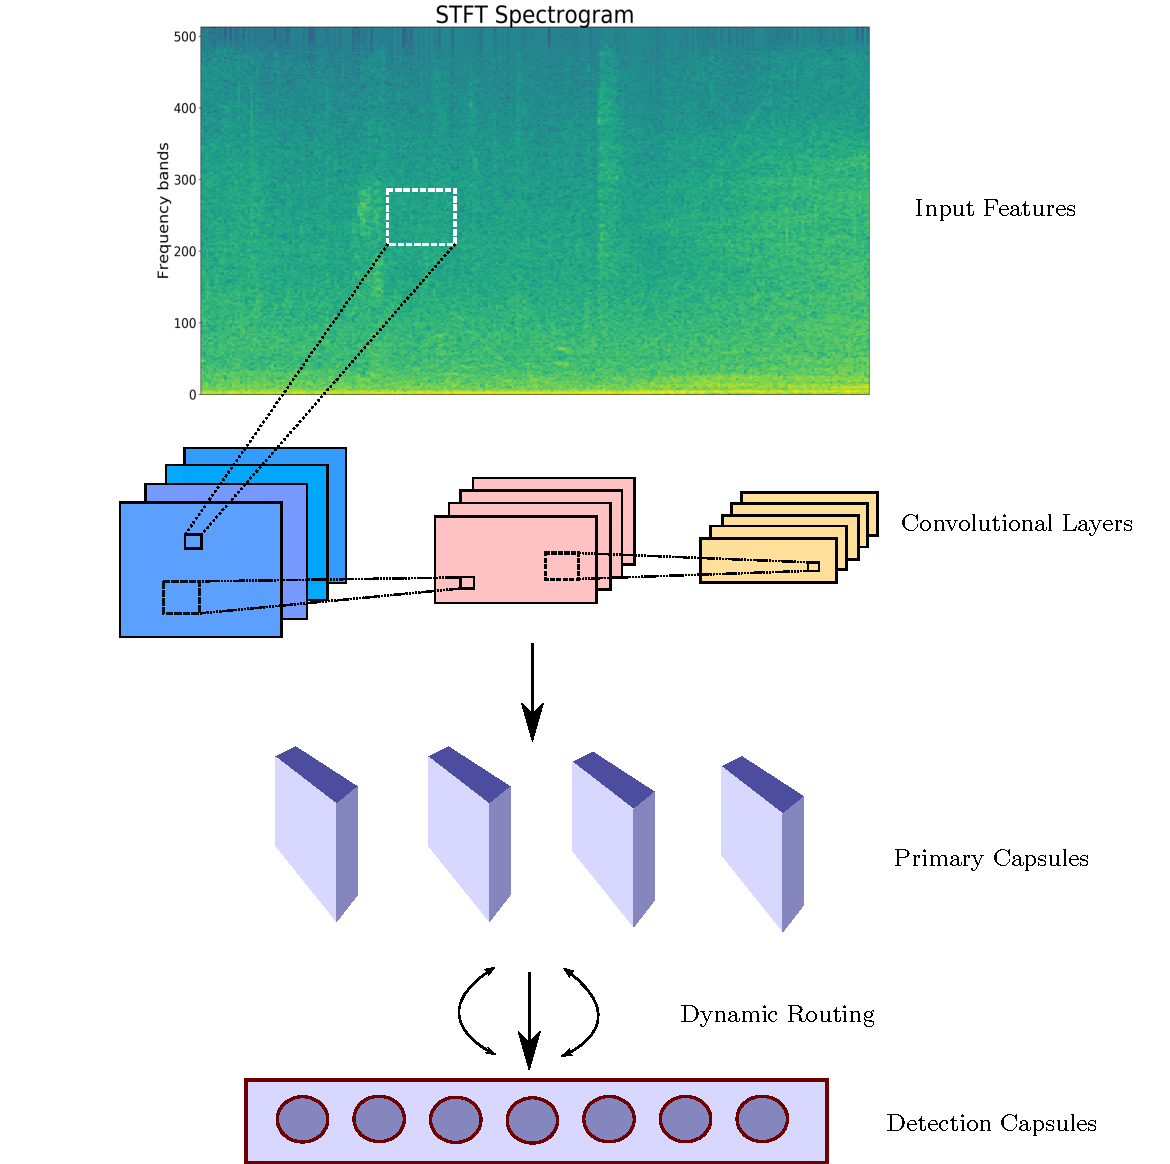
\includegraphics[width=\columnwidth]{img/flow_chart_2}
	\caption[Polyphonic SED with CapsNets]{Flow chart of the Capsule neural network architecture used for polyphonic sound event detection.}
	\label{fig:flowchart_capsulesed}
\end{figure}

In \cite{sabour2017dynamic}, the authors propose a series of densely connected neuron layers stacked at the bottom of the CapsNet, with the aim to regularize the weights training by reconstructing the input image $\mathbf{X} \in \mathbb{N}^{28 \times 28}$. Here, this technique entails an excessive complexity of the model to train, due to the higher number of units needed to reconstruct $\mathbf{X} \in \mathbb{R}^{T \times F \times C}$, yielding poor performance in our preliminary experiments. We decided, thus, to use dropout \cite{srivastava2014dropout} and $L_2$ weight normalization \cite{hoerl1970ridge} as regularization techniques, as done in \cite{iqbal2018capsule}.

\subsection{Experimental Setup}


In order to test the proposed method, we performed a series of experiments on three datasets provided to the participants of different editions of the DCASE challenge \cite{DCASE2017challenge, mesaros2016tut}. We evaluated the results by comparing the system based on the Capsule architecture with the traditional CNN. The hyperparameters of each network have been optimized with a \textit{random search} strategy \cite{bergstra2012random}. Furthermore, we reported the baselines and the best state-of-the-art performance provided by the challenge organizers.

\subsubsection{Dataset}


We assessed the proposed method on three datasets, two containing stereo recordings from real-life environments and one artificially generated monophonic mixtures of isolated sound events and real background audio.

In order to evaluate the proposed method in polyphonic real-life conditions, we used the TUT Sound Events 2016 \& 2017 datasets, which were included in the corresponding editions of the DCASE Challenge. For the monophonic-SED case study, we used the TUT Rare Sound Events 2017 which represents the task 2 of the DCASE 2017 Challenge.

\subsubsection{TUT Sound Events 2016}
The TUT Sound events 2016 (TUT-SED 2016)\footnote{\url{http://www.cs.tut.fi/sgn/arg/dcase2016/}} dataset consists of recordings from two acoustic scenes, respectively ``Home'' (indoor) and ``Residential area'' (outdoor) which we considered as two separate subsets. 
A total amount of around 54 and 59 minutes of audio are provided respectively for ``Home'' and ``Residential area'' scenarios.
Sound events present in each recording were manually annotated without any further cross-verification, due to the high level of subjectivity inherent to the problem. For further details, please refer to \secref{sec:dcase2016-dataset}.



\subsubsection{TUT Sound Events 2017}
The TUT Sound Events 2017 (TUT-SED 2017)\footnote{\label{note_dcase17}\url{http://www.cs.tut.fi/sgn/arg/dcase2017/}} dataset consists of recordings of street acoustic scenes with various levels of traffic and other activities, for a total of 121 minutes of audio. The scene was selected as representing an environment of interest for detection of sound events related to human activities and hazard situations. It is a subset of the TUT Acoustic scenes 2016 dataset \cite{mesaros2016tut}, from which also TUT-SED 2016 dataset was taken. Thus, the recording setup, the annotation procedure, the dataset splitting, and the cross-validation setup is the same described above. The 6 target sound event classes were selected to represent common sounds related to human presence and traffic, and they include brakes squeaking, car, children, large vehicle, people speaking, people walking. The evaluation set of the TUT-SED 2017 consists of 29 minutes of audio, whereas the development set is composed of 92 minutes of audio which are employed in the cross-validation procedure.

\subsubsection{TUT Rare Sound Events 2017} 
The TUT Rare Sound Events 2017 (TUT-Rare 2017)\textsuperscript{\ref{note_dcase17}} \cite{DCASE2017challenge} consists of isolated sounds of three different target event classes (respectively, baby crying, glass breaking and gunshot) and 30-second long recordings of everyday acoustic scenes to serve as background, such as park, home, street, cafe, train, etc. \cite{mesaros2016tut}. In this case we consider a \textit{monophonic}-SED, since the sound events are artificially mixed with the background sequences without overlap. For further details, please refer to \secref{sec:dcase-rare-2017-dataset}.

% In addition, the event potentially present in each test file is known a-priori thus it is possible to train different models, each one specialized for a sound event. In the development set, we used a number of sequences equal to 750, 750 and 1250 for training respectively of the baby cry, glass-break and gunshot models, while we used 100 sequences as validation set and 500 sequences as test set for all of them. In the evaluation set, the training and test sequences of the development set are combined into a single training set, while the validation set is the same used in the Development dataset. The system is evaluated against an ``unseen'' set of 1500 samples (500 for each target class) with a sound event presence probability for each class equal to 0.5.

%\subsection{Evaluation Metrics}
%
%In this work we used the Error Rate (ER) as primary evaluation metric to ensure comparability with the reference systems. In particular, for the evaluations on the TUT-SED 2016 and 2017 datasets we consider a segment-based ER with a one-second segment length, while for the TUT-Rare 2017 the evaluation metric is event-based error rate calculated using onset-only condition with a collar of 500 ms. 
%In the segment-based ER the ground truth and system output are compared in a fixed time grid, thus sound events are marked as active or inactive in each segment. For the event-based ER the ground truth and system output are compared at event instance level.
%
%ER score is calculated in a single time frame of one second length from intermediate statistics, i.e., the number of substitutions ($S(t_1)$), insertions ($I(t_1)$), deletions ($D(t_1)$) and active sound events from annotations ($N(t_1)$) for a segment $t_1$. Specifically:
%\begin{enumerate}
%	
%	\item Substitutions $S(t_1)$ are the number of ground truth events for which we have a false positive and one false negative in the same segment; %, thus: $S(t_1) = \min(FN(t_1),FP(t_1))$;
%	
%	\item Insertions $I(t_1)$ are events in system output that are not present in the ground truth, thus the false positives which cannot be counted as substitutions;%: $I(t_1) = \max(0,FN(t_1)-FP(t_1))$;
%	
%	\item Deletions $D(t_1)$ are events in ground truth that are not correctly detected by the system, thus the false negatives which cannot be counted as substitutions;%: $D(t_1)= \max(0,FP(t_1)-FN(t_1))$.
%	
%\end{enumerate}
%These intermediate statistics are accumulated over the segments of the whole test set to compute the evaluation metric ER. Thus, the total error rate is calculated as:
%\begin{equation}
%ER = \frac{\sum_{t_1=1}^{T} S(t_1) + \sum_{t_1=1}^{T} I(t_1) + \sum_{t_1=1}^{T} D(t_1)}{\sum_{t_1=1}^{T} N(t_1)},
%\end{equation}
%where $T$ is the total number of segments $t_1$.
%
%If there are multiple scenes in the dataset, such as in the TUT-SED 2016, evaluation metrics are calculated for each scene separately and then the results are presented as the average across the scenes.
%A detailed and visualized explanation of segment-based ER score in multi label setting can be found in \cite{mesaros2016metrics}.
%
%
\subsection{Comparative Algorithms}

Since the datasets we used were employed to develop and evaluate the algorithms proposed from the participants of the DCASE challenges, we can compare our results with the most recent approaches in the state-of-the-art. In addition, each challenge task came along with a baseline method that consists in a basic approach for the SED. It represents a reference for the participants of the challenges while they were developing their systems.

\subsubsection{TUT-SED 2016}
The baseline system is based on mel frequency cepstral coefficients (MFCC) acoustic features and multiple GMM-based classifiers. In detail, for each event class, a binary classifier is trained using the audio segments annotated as belonging to the model representing the event class, and the rest of the audio to the model which represents the negative class. The decision is based on likelihood ratio between the positive and negative models for each individual class, with a sliding window of one second.
To the best of our knowledge, the most performing method for this dataset is the algorithm we showed in \secref{sec:sed_dcase2016}.


\subsubsection{TUT-SED 2017}
In this case the baseline method relies on an MLP architecture using 40 LogMels as audio representation \cite{DCASE2017challenge}. The network is fed with a feature vector comprehending 5-frame as temporal context.
The neural network is composed of two dense layers of 50 hidden units per layer with the 20\% of dropout, while the network output layer contains $K$ sigmoid units (where $K$ is
the number of classes) that can be active at the same time and represent the network prediction of event activity for each context window.
The state of the art algorithm is based on the CRNN architecture \cite{adavanne2017report}. The authors compared both monaural and binaural acoustic features, observing that binaural features in general have similar performance as single channel features on the development dataset although the best result on the evaluation dataset is obtained using monaural LogMels as network inputs. According to the authors, this can suggest that the dataset was possibly not large enough to train the CRNN fed with this kind of features.

\subsubsection{TUT-Rare 2017}
The baseline \cite{mesaros2016tut} and the state-of-the-art methods of the DCASE 2017 challenge (Rare-SED) were based on a very similar architectures to that employed for the TUT-SED 2016 and described above. For the baseline method, the only difference relies in the output layer, which in this case is composed of a single sigmoid unit.
The first classified algorithm \cite{limrare} takes 128 LogMels as input and process them frame-wise by means of a CRNN with 1D filters on the first stage.


\subsection{Neural Network configuration}

%Since the size of the dataset usually affects the optimal network architecture, 
We performed a hyperparameter search by running a series of experiments over predetermined ranges. We selected the configuration that leads, for each network architecture, to the best results from the cross-validation procedure on the development dataset of each task, and used this architecture to compute the results on the corresponding evaluation dataset.

The number and shape of convolutional layers, the non-linear activation function, the regularizers in addition to the capsules dimensions and the maximum number of routing iterations have been varied for a total of 100 configurations. Details of searched hyperparameters and their ranges are reported in \tableref{tbl:hyper-params-capsule}.
The neural networks training was accomplished by the AdaDelta stochastic gradient-based optimization algorithm \cite{zeiler2012adadelta} for a maximum of 100 epochs and batch size equal to 20 on the margin loss function. The optimizer hyperparameters were set according to \cite{zeiler2012adadelta} (i.e., initial learning rate $lr=1.0$, $\rho=0.95$, $\epsilon=10^{-6}$). %It was chosen because it is well-suited for dealing with sparse data and its robustness to different choices of model hyperparameters. Furthermore no manual tuning of learning rate is required. 
The trainable weights were initialized according to the \textit{glorot-uniform} scheme \cite{glorot2010understanding} and an early stopping strategy was employed during the training in order to avoid overfitting. If the validation ER did not decrease for 20 consecutive epochs, the training was stopped and the last saved model was selected as the final model. In addition, dropout and $L_2$ weight normalization (with $\lambda=0.01$) have been used as weights regularization techniques \cite{srivastava2014dropout}. 
The algorithm has been implemented in the Python language using Keras \cite{chollet2015keras} and Tensorflow \cite{tensorflow2015-whitepaper} as deep learning libraries, while Librosa \cite{mcfee2015librosa} has been used for feature extraction.

\begin{table}[!t]
	\centering
	\begin{tabular} { lc c}
		\toprule
		Parameter & Range & Distribution\\  
		\midrule
		Batch Normalization  & [yes - no]	& random choice  \\
		\midrule
		
		CNN layers Nr.  & [1 - 4]& uniform \\
		
		CNN kernels Nr. & [4 - 64]& log-uniform \\
		
		CNN kernels dim. & [3$\times$3 - 8$\times$8]& uniform \\
		
		Pooling dim. & [1$\times$1 - 2$\times$5] & uniform 	\\
		
		CNN activation & [tanh - relu] & random choice \\
		
		CNN dropout  & [0 - 0.5]	& uniform  \\
		
		CNN L2  & [yes - no]	& random choice  \\		
		
		\midrule
		Primary Capsules Nr. $M$ & [2 - 8]	& uniform  \\
		
		Primary Capsules kernels dim. & [3$\times$3 - 5$\times$5]& uniform  \\
		
		Primary Capsules dimension $J$ & [2 - 16]	& uniform \\
		
		Detection Capsules dimension $G$ & [2 - 16]	& uniform \\
		
		Capsules dropout  & [0 - 0.5]	& uniform  \\
		
		Routing iterations  & [1 - 5]	& uniform \\
		
		\bottomrule
	\end{tabular}
	\caption[Polyphonic SED with CapsNets - Random Search]{Hyperparameters optimized in the random-search phase and the resulting best performing models.}		
	\label{tbl:hyper-params-capsule}
\end{table}

For the CNN models, we performed a similar random hyperparameters search procedure for each dataset, considering only the first two blocks of the \tableref{tbl:hyper-params-capsule} and by replacing the capsule layers with feedforward layers with \textit{sigmoid} activation function. 

On TUT-SED 2016 and 2017 datasets, the event activity probabilities are simply thresholded at a fixed value equal to 0.5, in order to obtain the binary activity matrix used to compute the reference metric. On the TUT-Rare 2017 the network output signal is processed as proposed in \cite{vesperini2018hierarchic}, thus it is convolved with an exponential decay window then it is processed with a sliding median filter with a local window-size and finally a threshold is applied.

\subsection{Results}
\label{sec:results}

In this section, we present the results for all the datasets and experiments described in \secref{sec:experiment}. The evaluation of Capsule and CNNs based methods have been conducted on the development sets of each examined dataset using random combinations of hyperparameters given in \tableref{tbl:hyper-params-capsule}. %As will be described in the following paragraphs, the CapsNets consistently outperform CNNs and baseline methods on in the case of Polyphonic-SED, while they pay a lack of generalization abilities in particular in the case of Mono-SED.

\subsection{TUT-SED 2016}
Results on TUT-SET 2016 dataset are shown in \tableref{tbl:results-dcase2016}, while \tableref{tbl:params-dcase2016} reports the configurations which yielded the best performance on the evaluation dataset. 
All the found models have ReLU as non-linear activation function and use dropout technique as weight regularization, while the batch-normalization applied after each convolutional layer seems to be effective only for the CapsNet. In \tableref{tbl:results-dcase2016} results are reported considering each combination of architecture and features we evaluated. The best performing setups are highlighted with bold face. The use of STFT as acoustic representation results to be beneficial for both the architectures with respect to the LogMels. In particular, the CapsNet obtains the lowest ER on the cross-validation performed on Development dataset when is fed by the binaural version of such features. On the two scenarios of the evaluation dataset, a model based on CapsNet and binaural STFT obtains an averaged ER equal to 0.69, which is largely below both the challenge baseline \cite{mesaros2016tut} (-0.19) and the best score reported in literature \cite{valenti2017neural} (-0.10). %, establishing a new state-of-the-art result. 
The comparative method based on CNNs seems not to fit at all when LogMels are used as input, while the performance is aligned with the challenge baseline based on GMM classifiers when the models are fed by monaural STFT. This discrepancy can be motivated by the enhanced ability of CapsNet to exploit small training datasets, in particular due to the effect of the routing mechanism on the weight training. In fact, the TUT-SED 2016 is composed of a small amount of audio and the sounds events occur sparsely (i.e., only 49 minutes of the total audio contain at least one event active), thus, the overall results of the comparative methods (CNNs, Baseline and SoA) on this dataset are quite low compared to the other datasets. 

Another CapsNet property that is worth to highlight is the lower number of free parameters that compose the models compared to evaluated CNNs.
As shown in \tableref{tbl:params-dcase2016}, the considered architectures have 267K and 252K free parameters respectively for the ``Home'' and the ``Residential area'' scenario. It is a relatively low number of parameters to be trained (e.g., a popular deep architecture for image classification such as AlexNet \cite{krizhevsky2012imagenet} is composed of 60M parameters), and the best performing CapsNets of each considered scenario have even less parameters with respect to the CNNs (-22\% and -64\%  respectively for the ``Home'' and the ``Residential area'' scenario). Thus, the high performance of CapsNet can be explained with the architectural advantage rather than the model complexity. In addition, there can be a significant performance shift for the same type of networks with the same number of parameters,
which means that a suitable hyperparameters search action (e.g., number of filters on the convolutional layers, dimension of the capsule units) is crucial in finding the best performing network structure.

\begin{table*}[h]
	\centering
	\resizebox{\textwidth}{!}{
		\begin{tabular}{@{}lllllll@{}}
			\toprule
			& \multicolumn{4}{c}{\textbf{TUT-SED 2016}}                                                                     & \multicolumn{2}{c}{\textbf{TUT-SED 2017}}             \\ \midrule
			& \multicolumn{2}{c}{Home}                              & \multicolumn{2}{c}{Residential}                       & \multicolumn{2}{c}{Street}                            \\ \midrule
			& \multicolumn{1}{c}{CapsNet} & \multicolumn{1}{c}{CNN} & \multicolumn{1}{c}{CapsNet} & \multicolumn{1}{c}{CNN} & \multicolumn{1}{c}{CapsNet} & \multicolumn{1}{c}{CNN} \\ \cmidrule(l){2-7} 
			CNN kernels Nr.               & $[32, 32, 8]$               & $[64,64,16,64]$         & $[4,16,32,4]$               & $[64]$                  & $[4,16,32,4]$               & $[64, 64,16, 64]$       \\
			CNN kernels dim.              & $6\times6$                  & $5\times5$              & $4\times4$                  & $5\times5$              & $4\times4$                  & $5\times5$              \\
			Pooling dim. ($F$ axis)       & $[4,3,2]$   				& $[2,2,2,2]$             & $[2,2,2,2]$                 & $[2]$             	  & $[2,2,2,2]$                 & $[2,2,2,2]$  			  \\
			MLP layers dim.               & -                           & $[85, 65]$              & -                           & $[42, 54, 66, 139]$     & -                           & $[85, 65]$              \\ \midrule
			Primary Capsules Nr. $M$ & 8                           & -				          & 7                           & -                       & 7                           & -                       \\
			Primary Capsules kernels dim. & $4\times4$                  & -                       & $3\times3$                  & -                       & $3\times3$                  & -                       \\
			Primary Capsules dimension   $J$ & 9                           & -                       & 16                          & -                       & 16                          & -                       \\
			Detection Capsules dimension         $G$   & 11                          & -                       & 8                           & -                       & 8                           & -                       \\
			Routing iterations            & 3                           & -                       & 4                           & -                       & 4                           & -                       \\
			\midrule
			\# Params                     & 267K                        & 343K                    & 252K                        & 709K                    & 223K                        & 342K                    \\ \bottomrule
		\end{tabular}
	}
	\caption[Polyphonic SED with CapsNets - Best models I]{Hyperparameters of the best performing models on the TUT-Polyphonic SED 2016 \& 2017 Evaluation datasets.}		
	\label{tbl:params-dcase2016}
\end{table*}


\begin{table*}[h]
	\centering
	\resizebox{\textwidth}{!}{
		\begin{tabular}{@{}lllllllll@{}}
			\toprule
			\multicolumn{9}{c}{\textbf{TUT-SED 2016 - Home}}                                                                                         \\ \midrule
			\multicolumn{5}{c|}{Development}                                                           & \multicolumn{4}{c}{Evaluation}                        \\ \midrule
			Features      & LogMels & Binaural  LogMels & STFT & \multicolumn{1}{l|}{Binaural STFT} & LogMels & Binaural LogMels & STFT & Binaural STFT \\ \midrule
			CNN           & 11.15     & 11.58              & 1.06 & \multicolumn{1}{l|}{1.07}        & 6.80      & 8.43               & 0.95 & 0.92       \\
			CapsNet      & 0.58      & 0.59               & 0.44 & \multicolumn{1}{l|}{\textbf{0.39}}        & 0.74      & 0.75               &\textbf{0.61} & 0.69        \\ \midrule
			\multicolumn{9}{c}{\textbf{TUT-SED 2016 - Residential Area}}                                                                             \\ \midrule
			Features      & LogMels & Binaural  LogMels & STFT & \multicolumn{1}{l|}{Binaural STFT} & LogMels & Binaural LogMels & STFT & Binaural STFT \\ \midrule
			CNN           & 3.24      & 3.11               & 0.64 & \multicolumn{1}{l|}{1.10}        & 2.36      & 2.76               & 1.00 & 1.35        \\
			CapsNet       & 0.36      & 0.34               & 0.32 & \multicolumn{1}{l|}{\textbf{0.32}}        & 0.72      & 0.75               & 0.78 &\textbf{0.68}        \\ \midrule
			\midrule
			\multicolumn{9}{c}{\textbf{TUT-SED 2016 - Averaged}}                                                                                         \\ \midrule
			CNN     & 7.20      & 7.35               & 0.85 & \multicolumn{1}{l|}{1.09}        & 4.58      & 5.60               & 0.98 & 1.14       \\
			CapsNet & 0.47      & 0.47               & 0.38 & \multicolumn{1}{l|}{\textbf{0.36}}        & 0.73      & 0.75               & 0.70 & \textbf{0.69}       \\
			\midrule
			Baseline \cite{mesaros2016tut}      & \multicolumn{4}{c|}{0.91}                                                & \multicolumn{4}{c}{0.88}                            \\
			SoA \cite{valenti2017neural}          & \multicolumn{4}{c|}{0.78}                                                & \multicolumn{4}{c}{0.79}                            \\ \bottomrule
			\toprule
			\multicolumn{9}{c}{\textbf{TUT-SED 2017}}                                                                                                                                  \\ \midrule
			& \multicolumn{4}{c|}{Development}                                                          & \multicolumn{4}{c}{Evaluation}                                      \\ \midrule
			Features & LogMels & Binaural  LogMels & STFT & \multicolumn{1}{l|}{Binaural STFT} & LogMels & Binaural LogMels & STFT & Binaural STFT \\ \midrule
			CNN      & 1.56             & 2.12                       & 0.57 & \multicolumn{1}{l|}{0.60}          & 1.38             & 1.79                      & 0.67 & 0.65        \\
			CapsNet  & 0.45             & 0.42                       & \textbf{0.36} & \multicolumn{1}{l|}{0.36} &\textbf{0.58}            & 0.64                      & 0.61 & 0.64 \\ 
			\midrule
			Baseline \cite{DCASE2017challenge} & \multicolumn{4}{c|}{0.69}							& \multicolumn{4}{c}{0.93} \\
			SoA \cite{adavanne2017report}     & \multicolumn{4}{c|}{0.52}             				& \multicolumn{4}{c}{0.79}  \\ \bottomrule
		\end{tabular}
	}
	\caption[Polyphonic SED with CapsNets - Results]{Results of best performing models in terms of ER on the TUT-SED 2016 \& 2017 dataset.}		
	\label{tbl:results-dcase2016}
\end{table*}


\subsubsection{Closer Look at Network Outputs}
A comparative study on the neural network outputs, which are regarded as event activity probabilities is presented in \figref{fig:activations}. The monaural STFT from a 40 seconds sequence of the ``Residential area'' dataset is shown along with event annotations and the network outputs of the CapsNet and the CNN best performing models. For this example, we chose the monaural STFT as input feature because generally it yields the best results over all the considered datasets. \figref{fig:activations} shows \textit{bird singing} lasting for the whole sequence and correctly detected by both the architectures. When the \textit{car passing by} event overlaps the \textit{bird singing}, the CapsNet detects more clearly its presence. The \textit{people speaking} event is slightly detected by both the models, while the \textit{object banging} activates the relative Capsule exactly only in correspondence of the event annotation. It must be noted that the dataset is composed of unverified manually labelled real-life recordings, that may present a degree of subjectivity, thus, affecting the training. Nevertheless, the CapsNet exhibits remarkable detection capability especially in the condition of overlapping events, while the CNN outputs are definitely more ``blurred'' and the event \textit{people walking} is wrongly detected in this sequence. 

\begin{figure}[h!]
	\centering
	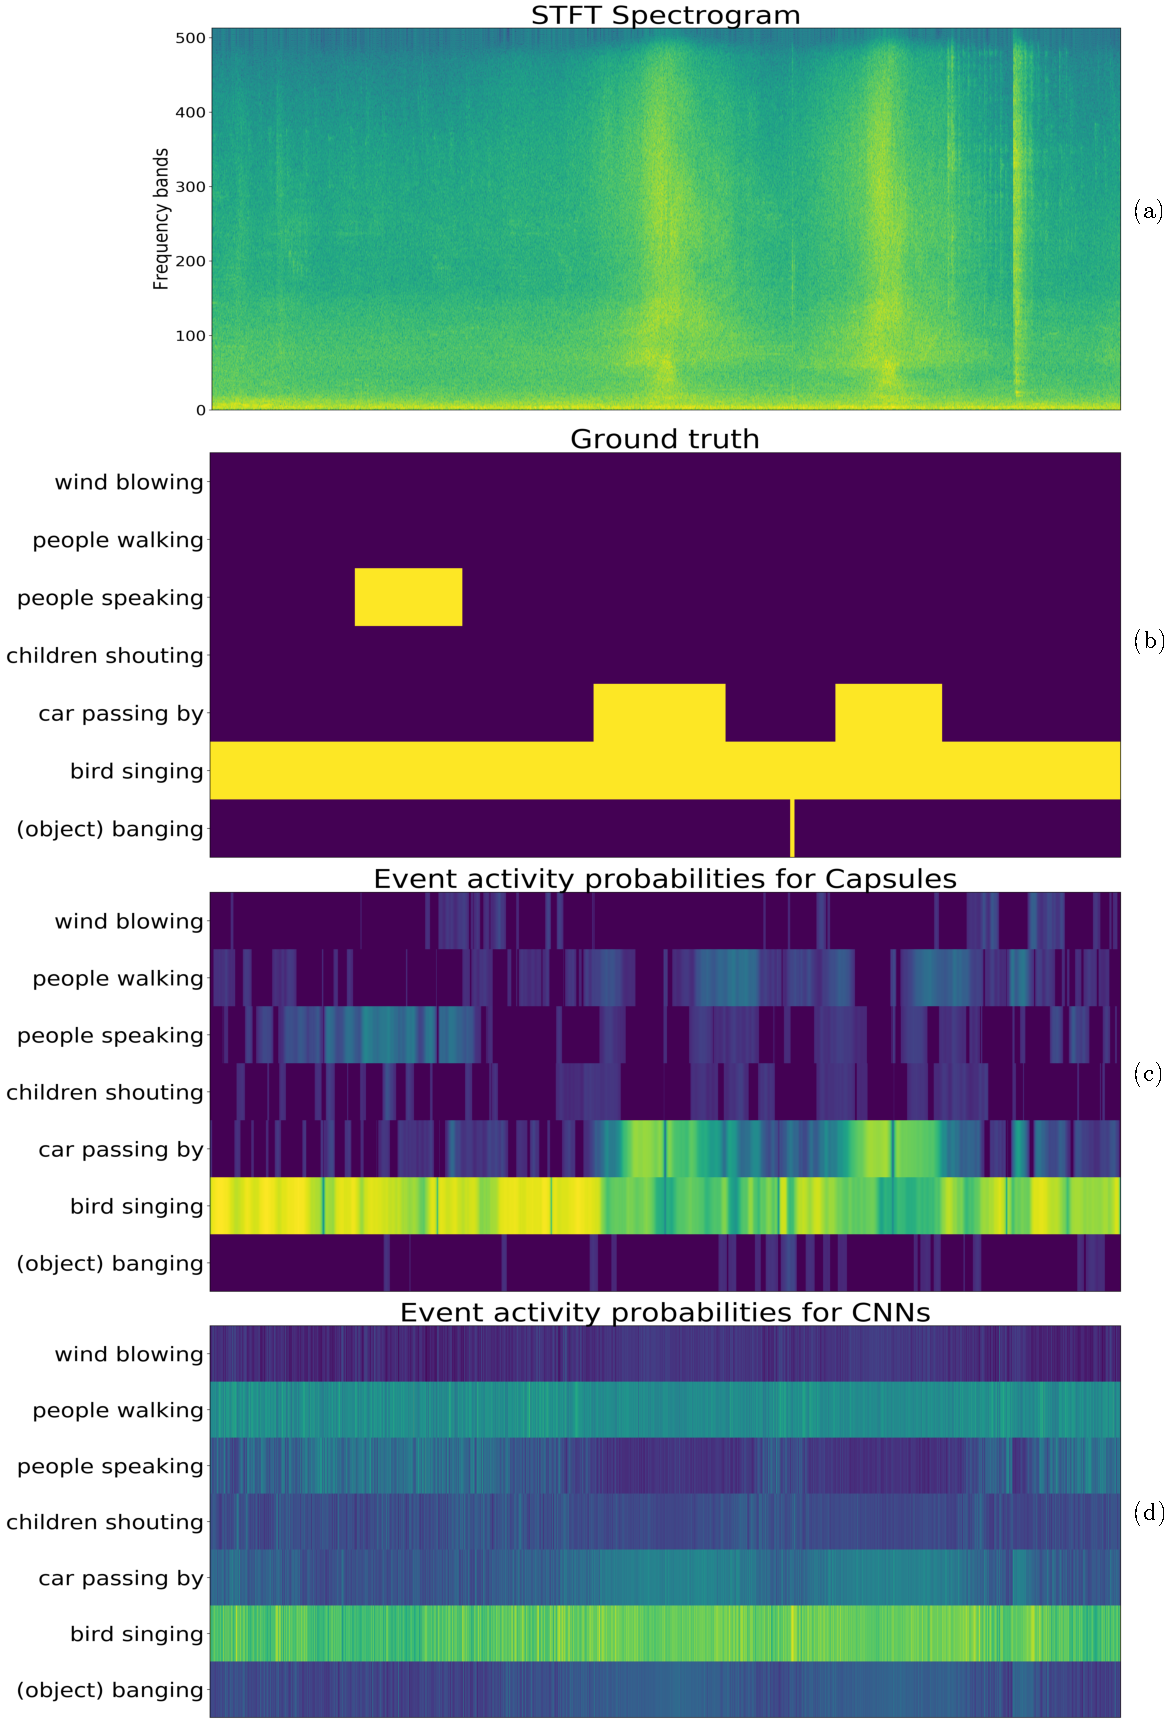
\includegraphics[width=0.5\columnwidth]{img/activations}
	\caption[Polyphonic SED - Network outputs I]{STFT Spectrogram of the input sequence (a), ground truth (b) and event activity probabilities for CapsNet (c) and CNN (d) from a sequence of test examples from TUT-SED 2016 dataset.}
	\label{fig:activations}
\end{figure}



\subsection{TUT-SED 2017}

The bottom of \tableref{tbl:results-dcase2016} reports the results obtained with the TUT-SED 2017. As in the TUT-SED 2016, the best performing models on the Development dataset are those fed by the Binaural STFT of the input signal. In this case we can also observe interesting performance obtained by the CNNs, which on the Evaluation dataset obtain a lower ER (i.e., equal to 0.65) with respect to the state-of-the-art algorithm \cite{adavanne2017report}, based on CRNNs. CapsNet confirms its effectiveness and it obtains lowest ER equal to 0.58 with LogMel features, although with a slight margin with respect to the other inputs (i.e., -0.03 compared to the STFT features, -0.06 compared to both the binaural version of LogMels and STFT spectrograms).

It is interesting to notice that in the development cross-validation, the CapsNet models yielded significantly better performance with respect to the other reported approaches, while the CNNs have decidedly worse performance. On the Evaluation dataset, it was not possible to use the early-stopping strategy, thus the ER scores of the CapsNets suffer more relative deterioration with respect to the CNNs scores, symptom of the sensibility of the CapsNets to the number of training iterations.

Notwithstanding this weakness, the absolute performance obtained both with monaural and binaural spectral features is consistent and improves the state-of-the-art result, with a reduction of the ER of up to 0.21 in the best case. This is particularly evident in \figref{fig:activations_17}, that shows the output of the two best performing systems for a sequence of approximately 20 seconds length which contains highly overlapping sounds. The event classes ``people walking'' and ``large vehicle'' are overlapped for almost all the sequence duration and they are well detected by the CapsNet, although they are of different nature: the ``large vehicle'' has a typical timber and is almost stationary, while the class ``people walking'' comprehend impulsive and desultory sounds. The CNN seems not to be able to distinguish between the ``large vehicle'' and the ``car'' classes, detecting confidently only the latter, while the activation corresponding ``people walking'' class is modest. The presence of the ``brakes squeaking'' class, which has a specific spectral profile mostly located in the highest frequency bands (as shown in the spectrogram), is detected only by the CapsNet. We can assume this as a concrete experimental validation of the routing effectiveness.

The number of free parameters amounts to 223K for the best configuration shown in \tableref{tbl:params-dcase2016} and it is similar to those found for the TUT-SED 2016, which consists also in this case in a reduction equal to 35\% with respect to the best CNN layout.

%\begin{table*}[!t]
%	\centering
%	\caption{Results of best performing models in terms of ER on the TUT-SED 2017 dataset.}		
%	\label{tbl:results-dcase2017}
%\begin{tabular}{@{}lllllllll@{}}
%	\toprule
%	\multicolumn{9}{c}{\textbf{TUT-SED 2017}}                                                                                                                                  \\ \midrule
%	& \multicolumn{4}{c|}{Development}                                                          & \multicolumn{4}{c}{Evaluation}                                      \\ \midrule
%	Features & LogMels & \textit{Binaural  LogMels} & STFT & \multicolumn{1}{l|}{Binaural STFT} & LogMels & Binaural LogMels & STFT & Binaural STFT \\ \midrule
%	CNN      & 1.56             & 2.12                       & 0.57 & \multicolumn{1}{l|}{0.60}          & 1.38             & 1.79                      & 0.67 & 0.65        \\
%	CapsNet  & 0.45             & 0.42                       & 0.36 & \multicolumn{1}{l|}{\textbf{0.36}} &\textbf{0.58}            & 0.64                      & 0.61 & 0.64 \\ 
%	\midrule
%	Baseline & \multicolumn{4}{c|}{0.69}							& \multicolumn{4}{c}{0.93} \\
%	SoA      & \multicolumn{4}{c|}{0.52}             				& \multicolumn{4}{c}{0.79}  \\ \bottomrule
%\end{tabular}
%\end{table*}




\begin{figure}[h]
	\centering
	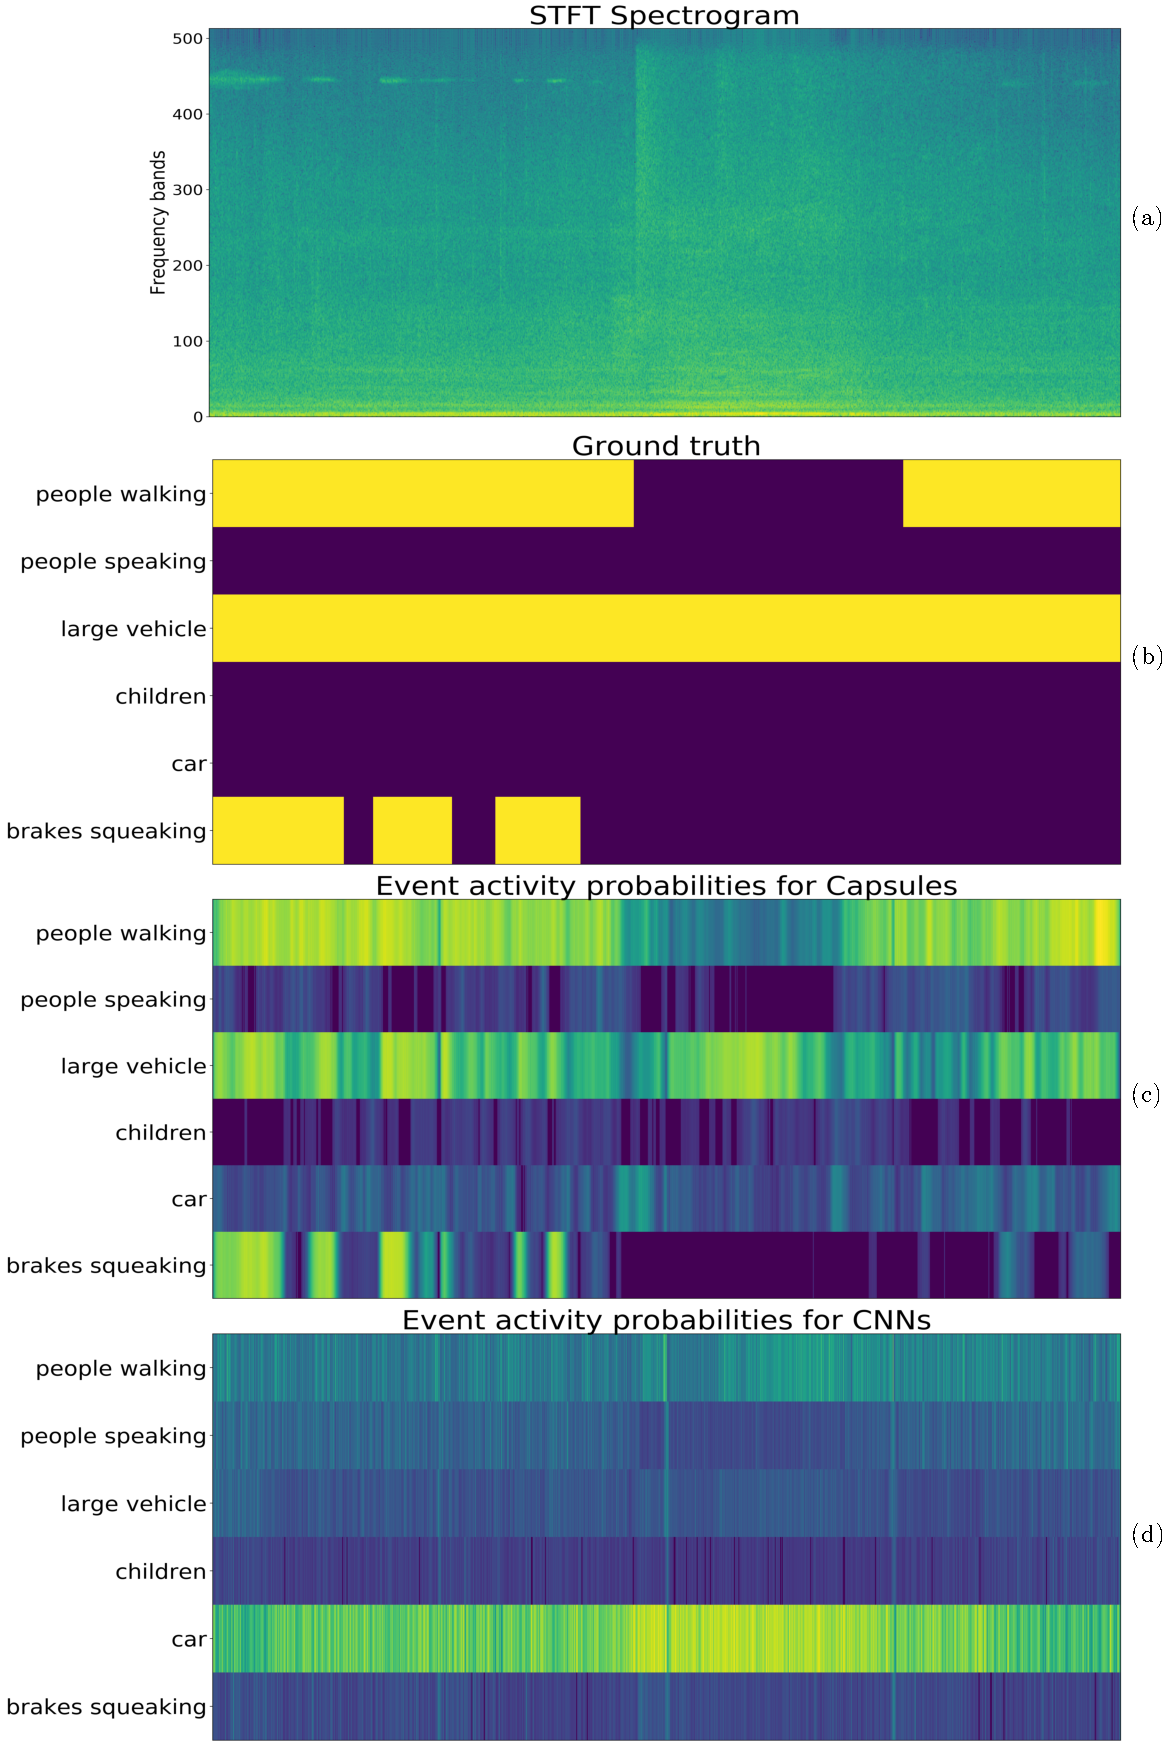
\includegraphics[width=0.5\columnwidth]{img/activations_17_v2}
	\caption[Polyphonic SED - Network outputs II]{STFT Spectrogram of the input sequence (a), ground truth (b) and event activity probabilities for CapsNet (c) and CNN (d) from a sequence of test examples from TUT-SED 2017 dataset.}
	\label{fig:activations_17}
\end{figure}

\subsection{TUT-Rare SED 2017}
The advantage given by the routing procedure to the CapsNet is particularly effective in the case of polyphonic SED. This is confirmed by the results obtained with the TUT-Rare SED 2017 which are shown in \tableref{tbl:results-dcase2017Rare}. In this case the metric is not anymore segment-based, but it is the event-based ER calculated using onset-only condition. We performed a separate random-search for each of the three sound event classes both for CapsNets and CNNs and we report the averaged score over the three classes. The setups that obtained the best performance on the Evaluation dataset are shown in \tableref{tbl:params-dcase2017-rare}. This is the largest dataset we evaluated and its characteristic is the high unbalance between the amount of background sounds versus the target sound events.

From the analysis of partial results on the Evaluation set (unfortunately not included for the sake of conciseness) we notice that both architectures achieve the best performance on \textit{glass break} sound (0.25 and 0.24 respectively for CNNs and CapsNet with LogMels features), due to its clear spectral fingerprint compared to the background sound. The worst performing class is the \textit{gunshot} (ER equal to 0.58 for the CapsNet), although the noise produced by different instances of this class involves similar spectral components. The low performance is probably motivated due to the fast decay of this sound, which means that in this case the routing procedure is not sufficient to avoid confusing the \textit{gunshot} with other background noises, especially in the case of dataset unbalancing and low event-to-background ratio. A solution to this issue can be find in the combination of CapsNet with RNN units, as proposed in \cite{cakir2017convolutional} for the CNNs which yields an efficient modelling of the \textit{gunshot} by CRNN and improves the detection abilities even in polyphonic conditions. The \textit{babycry} consists of short, harmonic sounds is detected almost equally from the two architectures due to the property of frequency shift invariance given by the convolutional kernel processing. 

Finally, the CNN shows better generalization performance to the CapsNet, although the ER score is far from state-of-the-art which involves the use of the aforementioned CRNNs \cite{limrare} or a hierarchical framework \cite{vesperini2018hierarchic}. In addition, in this case are the CNN models to have a reduced number of weights to train (36\%) with respect the CapsNets, except for the ``gunshot'' case but, as mentioned, it is also the configuration that gets the worst results.


\begin{table*}[h]
	\centering
	\resizebox{\textwidth}{!}{
		\begin{tabular}{@{}lllllll@{}}
			\toprule
			\multicolumn{7}{c}{\textbf{TUT-Rare SED 2017 Monophonic SED}}                                                                 \\ \midrule
			& \multicolumn{2}{c}{Babycry}   & \multicolumn{2}{c}{Glassbreak} & \multicolumn{2}{c}{Gunshot}  \\ \midrule
			& CapsNet      & CNN            & CapsNet       & CNN            & CapsNet    & CNN             \\ \cmidrule(l){2-7} 
			%Features                      & \multicolumn{6}{c}{LogMels}                                                          \\
			CNN kernels Nr.               & $[16,64,32]$ & $[16,32,8,16]$ & $[16,64,32]$  & $[16,32,8,16]$ & $[16,16]$  & $[16,64,32,32]$ \\
			CNN kernels dim.              & $6\times6$   & $8\times8$     & $6\times6$    & $8\times8$     & $8\times8$ & $7\times7$      \\
			Pooling dim. ($F$ axis)       & $[4,3,2]$    & $[3,3,2,2]$    & $[4,3,2]$     & $[3,3,2,2]$    & $[5,2]$    & $[5,4,2,1]$     \\
			MLP layers dim.               & -            & $[212,67]$     & -             & $[212,67]$     & -          & $112,51$        \\ \midrule
			Primary Capsules Nr. $M$& 7            & -               & 7             & -               & 8          & -                \\
			Primary Capsules kernels dim.  & $3\times3$   & -               & $3\times3$    & -               & $3\times3$ & -                \\
			Primary Capsules dimension  $J$  & 8            & -               & 8             & -               & 8          & -                \\
			Detection Capsules dimension      $G$      & 14           & -               & 14            & -               & 6          & -                \\
			Routing iterations            & 5            & -               & 5             & -              & 1          & -                \\ \midrule
			\# Params                     & 131K         & 84K            & 131K          & 84K            & 30K        & 211K            \\ \bottomrule
		\end{tabular}
	}
	\caption[Polyphonic SED with CapsNets - Best models II]{Hyperparameters of the best performing models on the TUT-Rare 2017 Monophonic SED Evaluation datasets.}		
	\label{tbl:params-dcase2017-rare}
\end{table*}

\begin{table}[h]
	\centering 
	\resizebox{0.75\textwidth}{!}{
	\begin{tabular}{@{}lllll@{}}
		\toprule
		\multicolumn{5}{c}{\textbf{TUT-RareSED 2017 - Monophonic SED}}                           \\ \midrule
		& \multicolumn{2}{c|}{Development}             & \multicolumn{2}{c}{Evaluation} \\ \midrule
		Features & LogMels & \multicolumn{1}{l|}{STFT} & LogMels     & STFT    \\
		CNN      & 0.29             & \multicolumn{1}{l|}{0.21} & \textbf{0.41}        & 0.46    \\
		CapsNet  & \textbf{0.17}    & \multicolumn{1}{l|}{0.20} & 0.45                 & 0.54    \\
		\hline
		Baseline \cite{mesaros2016tut} & 0.53             & \multicolumn{1}{l|}{}     & 0.64                &         \\	
		Hierarchic CNNs  \cite{vesperini2018hierarchic}   & 0.13             & \multicolumn{1}{l|}{}     & 0.22                 &         \\
		SoA  \cite{limrare}    &\textbf{0.07}             & \multicolumn{1}{l|}{}     &\textbf{0.13}                 &         \\ \bottomrule
	\end{tabular}
	}
	\caption[Polyphonic SED with CapsNets - Results II]{Results of best performing models in terms of ER on the TUT-RareSED 2017 dataset.}		
	\label{tbl:results-dcase2017Rare}
\end{table}

\subsection{Alternative Dynamic Routing for SED}
We observed that the original routing procedure implies the initialization of the coefficients $\beta_{ij}$ to zero each time the procedure is restarted, i.e, after each input sample has been processed. This is reasonable in the case of image classification, for which the CapsNet has been originally proposed. In the case of audio task, we clearly expect a higher correlation between samples belonging to adjacent temporal frames $\mathbf{X}$. We thus investigated the chance to initialize the coefficients $\beta_{ij}$ to zero only at the very first iteration, while for subsequent $\mathbf{X}$ to assign them the last values they had at the end of the previous iterative procedure. We experimented this variant considering the best performing models of the analyzed scenarios for polyphonic SED, taking into account only the systems fed with the monaural STFT. As shown in \tableref{tbl:results-new-routing}, the modification we propose in the routing procedure is effective in particular on the evaluation datasets, conferring improved generalization properties to the models we tested even without accomplishing a specific hyperparameters optimization. %. An further hyper-parameter optimization could improve the results, but we did not perform it because our goal was to establish the method effectiveness.


\begin{table}[ht]
	\centering 
	\begin{tabular}{@{}lllll@{}}
		\toprule
		\multicolumn{5}{c}{\textbf{TUT-SED 2016 - Home}}                                   \\ \midrule
		& \multicolumn{2}{c|}{Development}   & \multicolumn{2}{c}{Evaluation} \\ \midrule
		CapsNet      & 0.44 & \multicolumn{1}{l|}{}       & 0.61              &            \\
		CapsNet - NR & 0.41 & \multicolumn{1}{l|}{-6.8\%} & \textbf{0.58}     & -4.9 \%    \\ \midrule
		\multicolumn{5}{c}{\textbf{TUT-SED 2016 - Residential}}                            \\ \midrule
		CapsNet      & 0.32 & \multicolumn{1}{l|}{}       & 0.78              &            \\
		CapsNet - NR & 0.31 & \multicolumn{1}{l|}{-3.1\%} & \textbf{0.72}     & -7.7 \%    \\ \midrule
		\multicolumn{5}{c}{\textbf{TUT-SED 2016 - Average}}                                \\ \midrule
		CapsNet      & 0.38 & \multicolumn{1}{l|}{}       & 0.70              &            \\
		CapsNet - NR & 0.36 & \multicolumn{1}{l|}{-5.3\%} & \textbf{0.65}     & -7.1 \%    \\ \midrule
		\multicolumn{5}{c}{\textbf{TUT-SED 2017 - Street}}                                 \\ \midrule
		CapsNet      & 0.36 & \multicolumn{1}{l|}{}       & 0.61              &            \\
		CapsNet - NR & 0.36 & \multicolumn{1}{l|}{-0.0\%} & \textbf{0.58}     & -4.9 \%    \\ \bottomrule
	\end{tabular}
	\caption[Polyphonic SED with CapsNets - Alternative routing]{Results of test performed with our proposed variant of routing procedure.}		
	\label{tbl:results-new-routing}
\end{table}

\subsection{Conclusion}
\label{sec:conclusions}
In this work, we proposed to apply the CapsNet architecture to the polyphonic SED task. 

Part of the novelty of this work resides in the adaptation of the CapsNet architecture for the audio event detection task, with a special care on the input data, the layers interconnection and the regularization techniques. The routing procedure is also modified to confer a more appropriate acoustic rationale, with a further average performance improvement of 6\% among the polyphonic-SED tasks.

An extensive evaluation of the algorithm is proposed with comparison to recent state-of-the-art methods on three different datasets. The experimental results demonstrate that the use of dynamic routing procedure during the training is effective and provides significant performance improvement in the case of overlapping sound events compared to traditional CNNs, and other established methods in polyphonic SED. Interestingly, the CNN based method obtained the best performance in the monophonic SED case study, thus emphasizing the suitability of the CapsNet architecture in dealing with overlapping sounds.
We showed that this model is particularly effective with small sized datasets, such as TUT-SED 2016 which contains a total 78 minutes of audio for the development of the models of which one third is background noise.
Furthermore, the network trainable parameters are reduced with respect to other deep learning architectures, confirming the architectural advantage given by the introduced features also in the task of polyphonic SED. 
Despite the improvement in performance, we identified a limitation of the proposed method. As presented in \secref{sec:results}, the performance of the CapsNet is more sensible to the number of training iterations. This affects the generalization capabilities of the algorithm, yielding a greater relative deterioration of the performance on evaluation datasets with respect to the comparative methods.

The results we observed in this work are consistent with many other classification tasks in various domains \cite{deng2018hyper, shen2018dynamic, jalal2018american}, prove that the CapsNet is an effective approach which enhances the well-established representation capabilities of the CNNs also in the audio field. As a future work, regularization methods can be investigated to overcome the lack of generalization which seems to affect the CapsNets. Furthermore, regarding the SED task the addition of recurrent units may be explored to enhance the detection of particular (i.e., inpulsive) sound events in real-life audio and the recently-proposed variant of routing, based on the Expectation Maximization algorithm (EM) \cite{hinton2018matrix}, can be investigated in this context.
